\documentclass[cropped,10pt]{standalone}

\usepackage{tikz}

% helvetica font
\usepackage[scaled=1.1]{helvet}
\usepackage{sfmath}
\renewcommand{\familydefault}{\sfdefault}

% or comment out previous 3 lines, and uncomment the one below, for clean latex font
%\usepackage{cmbright}

% you might want to define some colors:
%\definecolor{myred}{HTML}{E51E10}
%\definecolor{myblue}{HTML}{56B4E9}

\usetikzlibrary[positioning,arrows,arrows.meta,shapes,calc,spy,intersections,shadows,bending]
\usetikzlibrary[decorations.text,decorations.pathmorphing,decorations.markings]

\pagestyle{empty}
\thispagestyle{empty}

\begin{document}

\begin{tikzpicture}

% ----------------------------------------------------



% ----------------------------------------------------

% HERE YOU CAN USE TIKZ CODE TO ADD DIAGRAMS ETC

% don't forget all your panel labels etc
% e.g.:
% \node at (10,90) [anchor=base,font=\bfseries,scale=1.5] {A};
  \node at (0, 99) [anchor = north west] {
  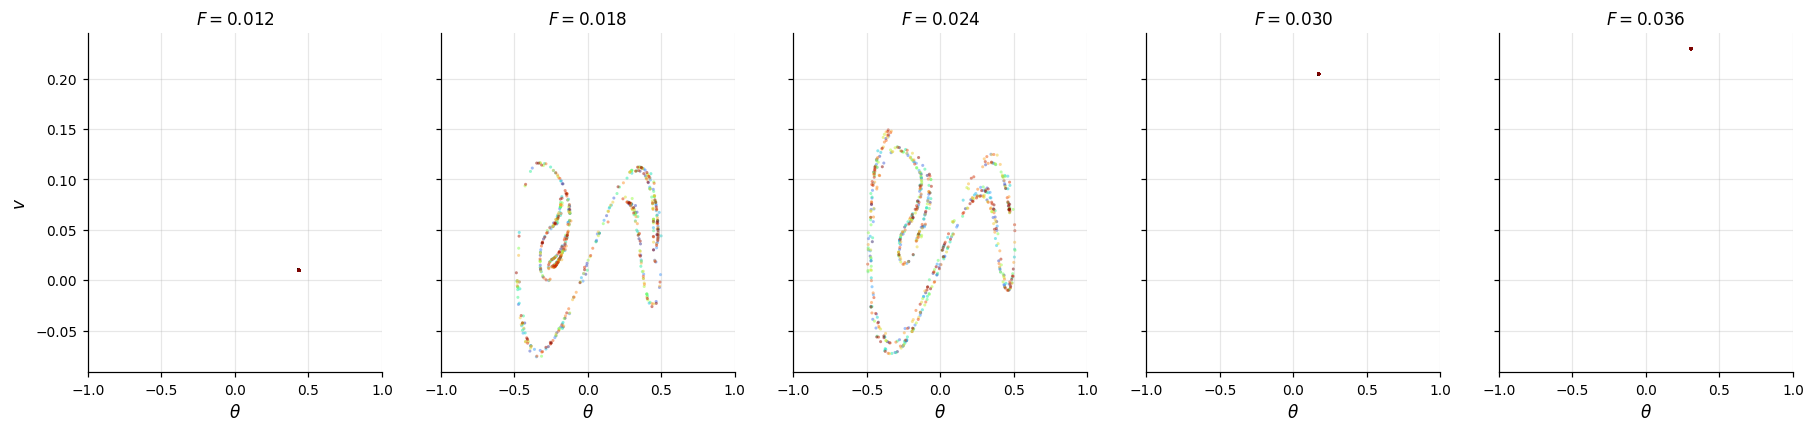
\includegraphics{../figures_melnikov/duffing_poincare.png}
  };
  \node at (0, 88) [anchor = north west] {
  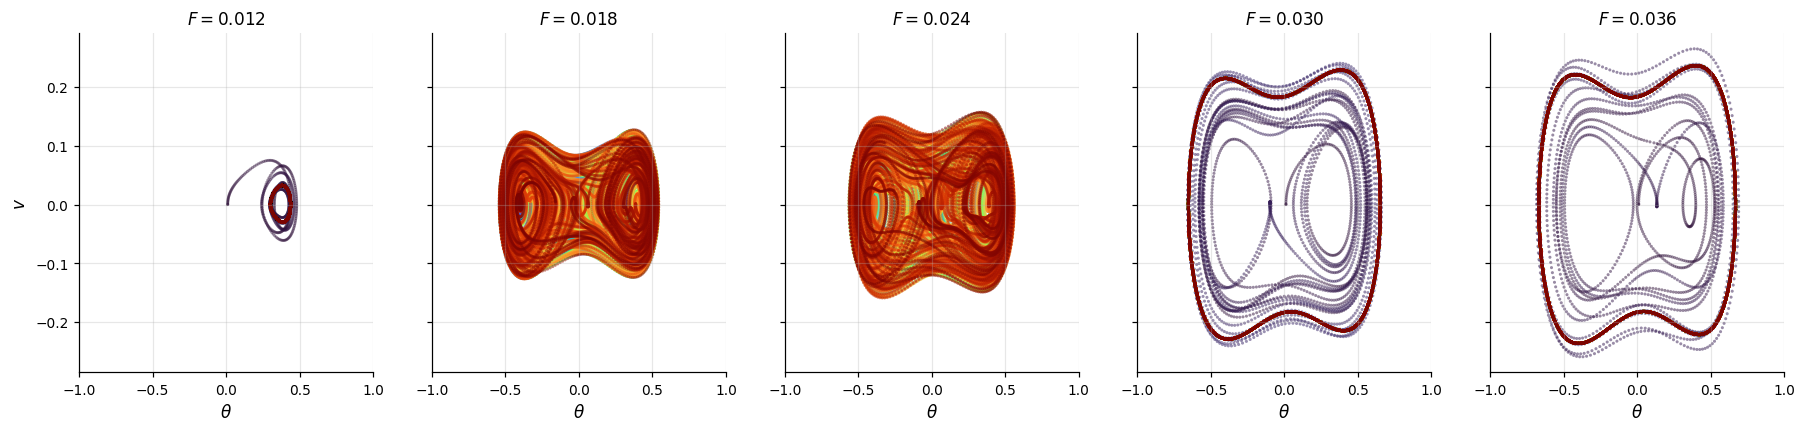
\includegraphics{../figures_melnikov/duffing_poincare_traj.png}
  };
  \node at (42, 88) [anchor = north west] {
  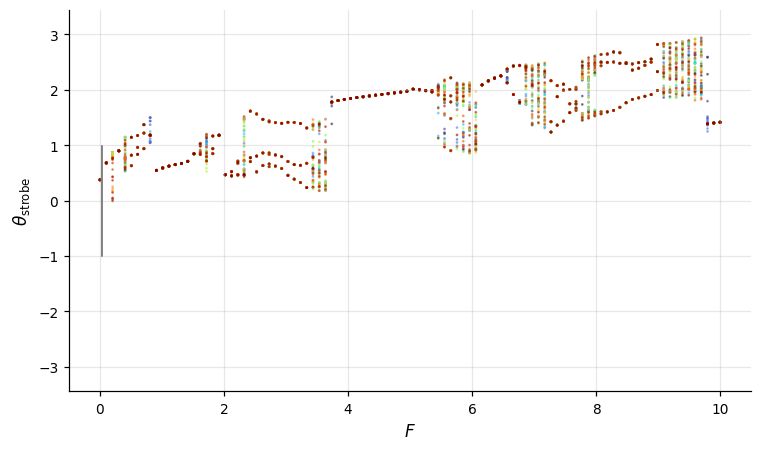
\includegraphics{../figures_melnikov/figure_bif_duff_long.png}
  };
  \node at (42, 99) [anchor = north west] {
  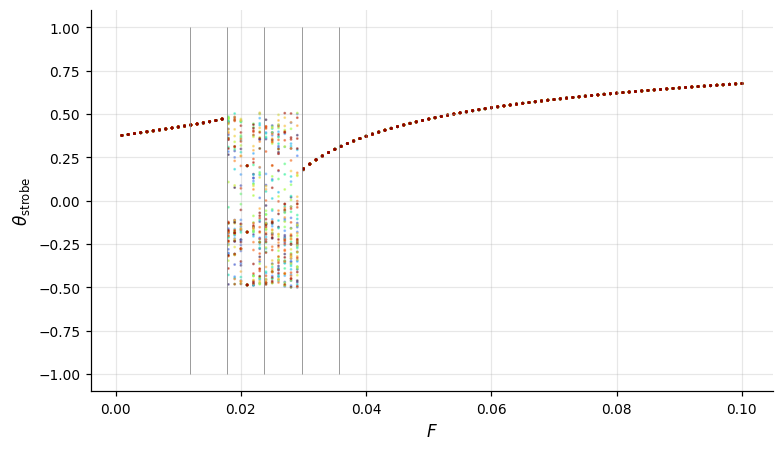
\includegraphics{../figures_melnikov/figure_bif_duff.png}
  };
  \node at (42, 77) [anchor = north west] {
  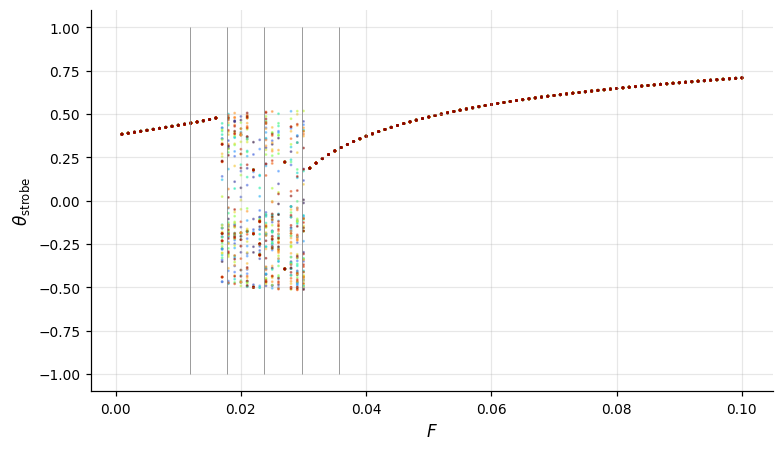
\includegraphics{../figures_melnikov/figure_bif_pfl3.png}
  };
  \node at (42, 66) [anchor = north west] {
  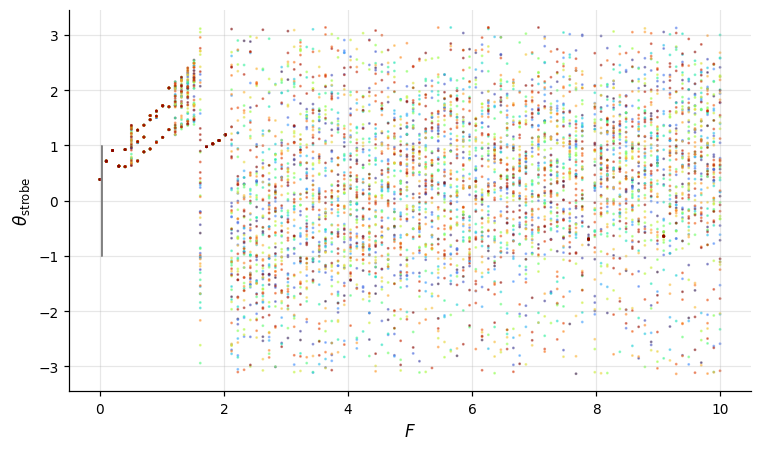
\includegraphics{../figures_melnikov/figure_bif_pfl3_long.png}
  };
  \node at(0, 100)[anchor = north, font = \bfseries, scale = 3]{A};
  \node at(1, 99.5)[anchor = north, font = \bfseries, scale = 2]{i};
  \node at(43, 99.5)[anchor = north, font = \bfseries, scale = 2]{ii};
  \node at(1, 88.5)[anchor = north, font = \bfseries, scale = 2]{iii};
  \node at(43, 88.5)[anchor = north, font = \bfseries, scale = 2]{iv};

  \node at (0, 77) [anchor = north west] {
  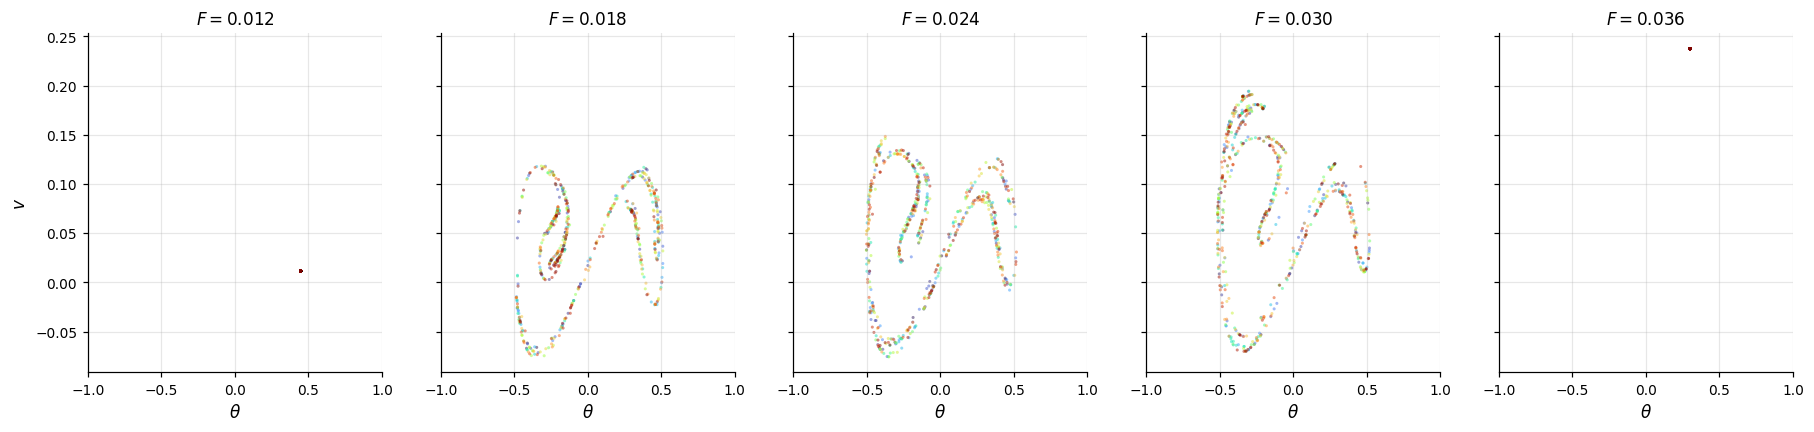
\includegraphics{../figures_melnikov/pfl3_12_poincare.png}
  };
  \node at (0, 66) [anchor = north west] {
  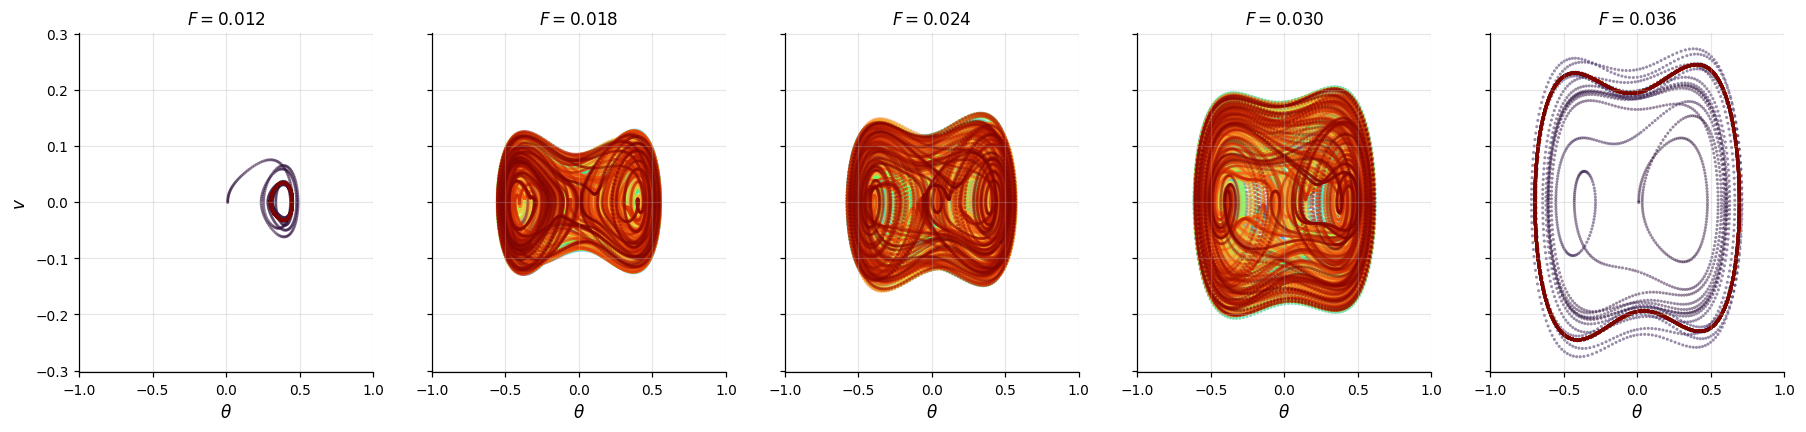
\includegraphics{../figures_melnikov/pfl3_12_poincare_traj.png}
  };
  \node at(0, 78)[anchor = north, font = \bfseries, scale = 3]{B};
  \node at(1, 77.5)[anchor = north, font = \bfseries, scale = 2]{i};
  \node at(1, 66.5)[anchor = north, font = \bfseries, scale = 2]{iii};
  \node at(43, 77.5)[anchor = north, font = \bfseries, scale = 2]{ii};
  \node at(43, 66.5)[anchor = north, font = \bfseries, scale = 2]{iv};


  \node at (0, 55) [anchor = north west] {
  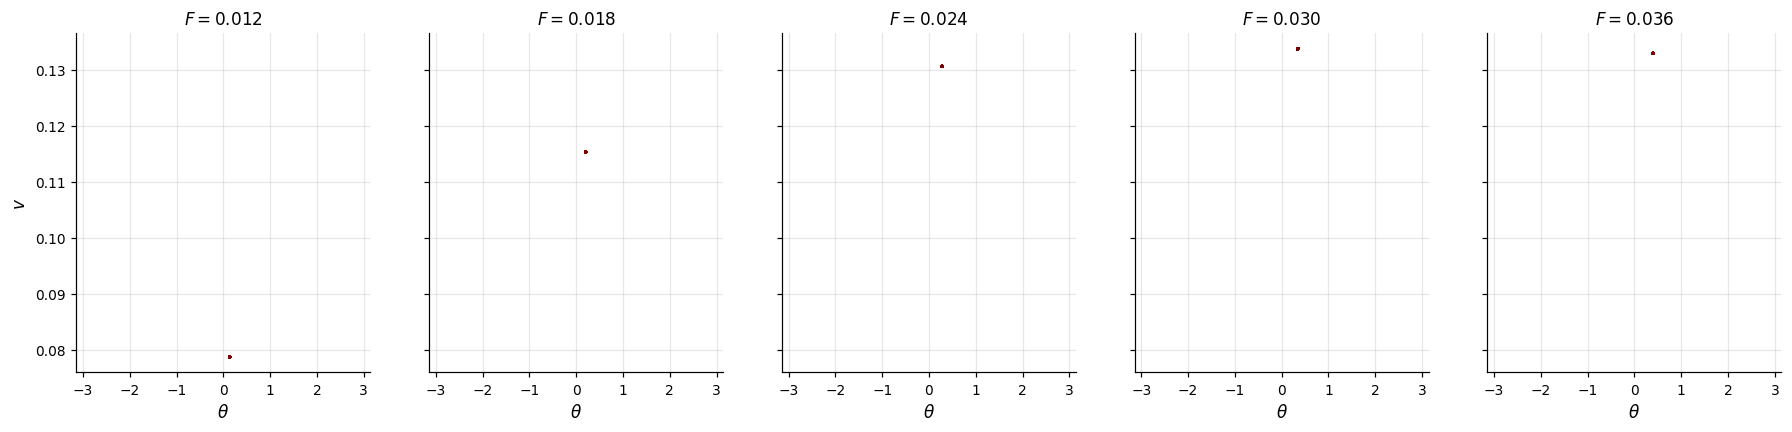
\includegraphics{../figures_melnikov/pfl3_6_poincare.png}
  };
  \node at (0, 44) [anchor = north west] {
  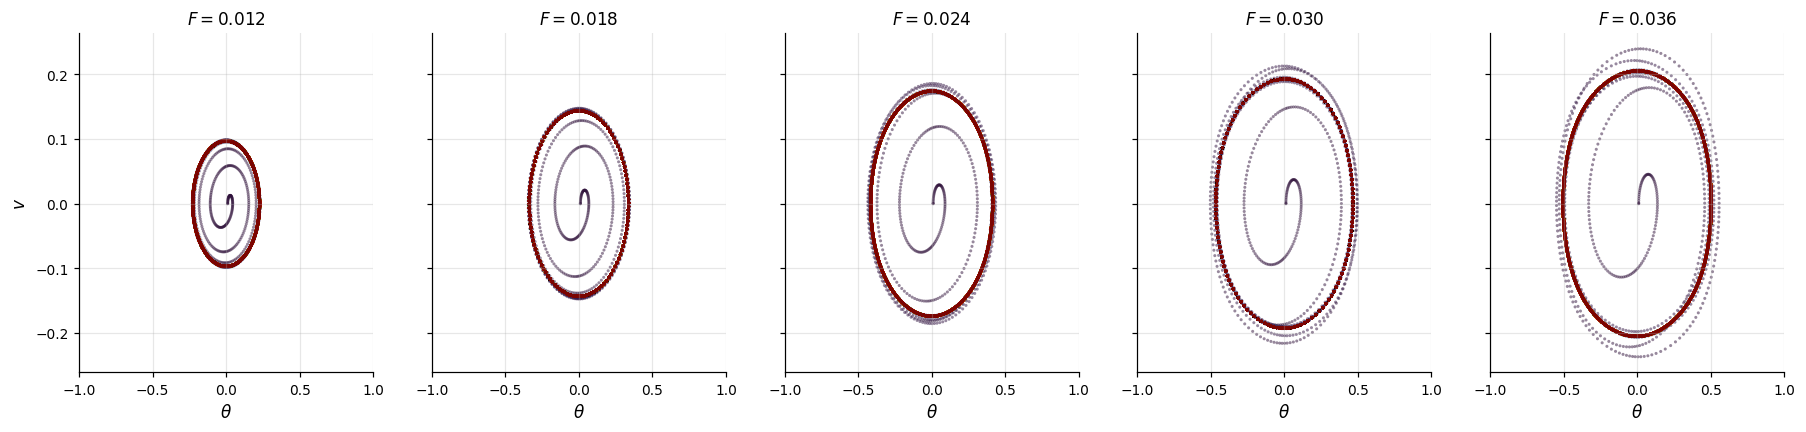
\includegraphics{../figures_melnikov/pfl3_6_poincare_traj.png}
  };
  \node at (42, 55) [anchor = north west]{
  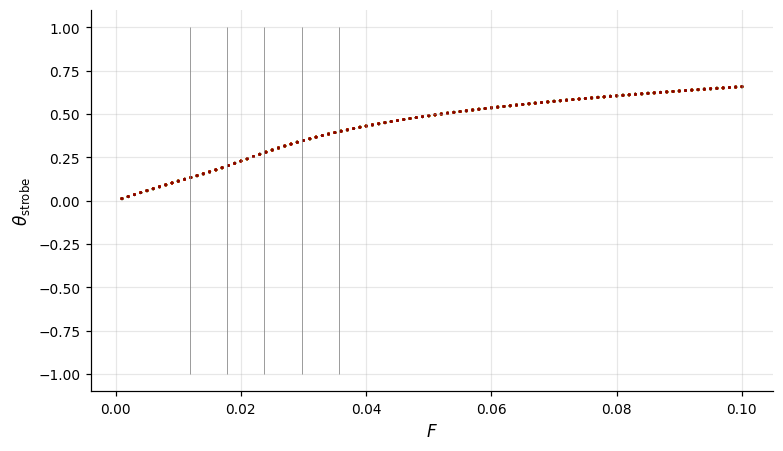
\includegraphics{../figures_melnikov/figure_bif_pfl3_6.png}
  };
  \node at (42, 44) [anchor = north west] {
  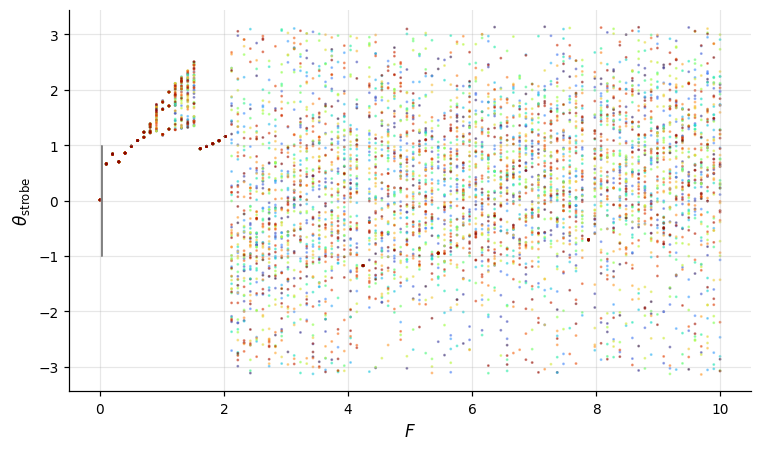
\includegraphics{../figures_melnikov/figure_bif_pfl3_6_long.png}
  };
  \node at(0, 56)[anchor = north, font = \bfseries, scale = 3]{C};
  \node at(1, 55.5)[anchor = north, font = \bfseries, scale = 2]{i};
  \node at(1, 44.5)[anchor = north, font = \bfseries, scale = 2]{iii};
  \node at(43, 55.5)[anchor = north, font = \bfseries, scale = 2]{ii};
  \node at(43, 44.5)[anchor = north, font = \bfseries, scale = 2]{iv};
  \draw [black, very thick, dashed] (50, 90.3) -- (44.6, 84.5);
  \draw [black, very thick, dashed] (46.5, 90.3) -- (44.6, 84.5);
  \draw [black, very thick, dashed] (50, 68.3) -- (44.6, 62.5);
  \draw [black, very thick, dashed] (46.5, 68.3) -- (44.6, 62.5);
  \draw [black, very thick, dashed] (50, 46.3) -- (44.6, 40.5);
  \draw [black, very thick, dashed] (46.5, 46.3) -- (44.6, 40.5);
% helper grid (comment out once you're done!)
%\draw[help lines,step=1,thin,gray!20] (0,0) grid (100, 100);
%\draw[help lines,step=5,gray!20,very thick] (0,0) grid (100, 100);
%\draw[help lines,step=10,gray!40,ultra thick] (0,0) grid (100, 100);
%
%\foreach \j in {10,15,..., 50}
%  \node at (\j,85) [fill=white,text=red!80!black] {\j};
%\foreach \j in {10,15,..., 95}
%  \node at (23,\j) [fill=white,text=green!80!black] {\j};
\end{tikzpicture}
\end{document}

